\section{Fill between}
\label{sec:fillbetween}
\begin{pgfplotslibrary}{fillbetween}
	The |fillbetween| library allows to fill the area between two arbitrary named plots.
	It can also identify segments of the intersections and fill the segments individually.
\end{pgfplotslibrary}

\begingroup
\pgfkeys{
	/pgfmanual/gray key prefixes/.add={}{,/tikz/fill between/},
	/pdflinks/search key prefixes in/.add={}{,/tikz/fill between/},
}

\subsection{Filling an Area}
\begin{addplotoperation}[]{fill between}{[\marg{options defined with prefix \normalfont\texttt{/tikz/fill between}}]}
	A special plotting operation which takes two named paths on input and generates one or more paths resembling the filled area between the input paths.

\begin{codeexample}[]
\begin{tikzpicture}
\begin{axis}
	\addplot+[name path=A,domain=0:1,samples=2] {x};

	\addplot+[name path=B] table {
		x y
		0 2
		0.5 -1
		1 3
	};

	\addplot fill between[of=A and B];
\end{axis}
\end{tikzpicture}
\end{codeexample}
	The operation |fill between| requires at least one input key within \meta{options defined with prefix \normalfont\texttt{/tikz/fill between}}: the two involved paths in the form |of=|\meta{first}| and |\meta{second}. Here, both \meta{first} and \meta{second} need to be defined using |name path| (or |name path global|). The arguments can be exchanged\footnote{Note that some options refer explicitly to either the first or the second input path. These options are document accordingly.}, i.e.\ we would archieve the same effect for |of=B and A|.

	The argument \meta{options defined with prefix \normalfont\texttt{/tikz/fill between}} can contain any number of options which have the prefix |/tikz/fill between|. Note that the prefix refers to the reference manual, you do not need to type the prefix. This excludes drawing options like |fill=orange|; these options should be given as \meta{options} (or inside of styles like |every segment|). Allowed options include |of|, |split|, |soft clip|, and style definitions of |every segment| and its friends, i.e.\ those which define which paths are to be acquired and how they should be processed before they can be visualized.

	A |fill between| operation takes the two input paths, analyzes their orientation (i.e.\ are its coordinates given increasing in $x$ direction?), connects them, and generates a |fill| path. 
	
	As mentioned above, the input paths need to be defined in advance (forward references are unsupported). If you would generate the filled path manually, you would draw it \emph{before} the other ones such that it does not overlap. This is done implicitly by \PGFPlots: as soon as \PGFPlots\ encounteres a |fill between| plot, it will activate layered graphics. The filled path will be placed on layer \declareandlabel{pre main} which is between the main layer and the background layer.\label{Layer!pre main} 

	A |fill between| operation is just like a usual plot: it makes use of the |cycle list|, i.e.\ it receives default plot styles. Our first example above uses the default |cycle list| which has a brown color. We can easily redefine the appearance just as for any other plot by adding options in square braces:
\begin{codeexample}[]
\begin{tikzpicture}
\begin{axis}
	\addplot[blue,name path=A,domain=0:1] {sqrt(x)};

	\addplot[red, name path=B,domain=0:1] {sqrt(x/2)};

	\addplot[gray] fill between[of=A and B];
\end{axis}
\end{tikzpicture}
\end{codeexample}

	Note that the number of data points does not restrict |fill between|. In particular, you can combine different arguments easily.
\begin{codeexample}[]
\begin{tikzpicture}
\begin{axis}
	\addplot[blue,name path=A,domain=0:1] 
		{sin(360*x)};

	\addplot[red, name path=B,domain=0:1,samples=2] 
		{0.5};

	\addplot[orange] fill between[of=A and B];
\end{axis}
\end{tikzpicture}
\end{codeexample}

The combination of input plots is also possible if one or both of the plots make use of |smooth| interpolation:
\begin{codeexample}[]
\begin{tikzpicture}
\begin{axis}
	\addplot+[name path=A,samples=7,smooth,domain=0:1] 
		{sin(360*x)};

	\addplot+[name path=B,samples=15,domain=0:1]
		{cos(360*x)};

	\addplot[orange] fill between[of=A and B];
\end{axis}
\end{tikzpicture}
\end{codeexample}

	Actually, a |fill between| path operates directly on the low--level input path segments. As such, it is much closer to, say, a \Tikz\ decoration than to a plot; only its use-cases (legends, styles, layering) are tailored to the use as a plot. However, the input paths can be paths and/or plots. The example below combines one |\addplot| and one |\path|.
\begin{codeexample}[]
\begin{tikzpicture}
\begin{axis}[ymin=-0.2,enlargelimits]
	\addplot+[name path=A,smooth] 
		coordinates {(0,0) (1,1) (2,0)};

	\path[name path=B]
		(axis cs:0.5,-0.2) -- (axis cs:1.8,-0.2);

	\addplot[orange] fill between[of=A and B];
\end{axis}
\end{tikzpicture}
\end{codeexample}
	
	As mentioned above, |fill between| takes the two input paths as such and combines them to a filled segment. To this end, it connects the end--points of both paths. This can be seen in the example above: the path named `|B|' has different $x$ coordinates than `|A|' and results in a trapezoidal output.

	
	Here is another example in which a plot and a normal path are combined using |fill between|. Note that the |\draw| path is generated using nodes of path `|A|'. In such a scenario, we may want to fill only the second segment which is also possible, see |split| below.
\begin{codeexample}[]
\begin{tikzpicture}
\begin{axis}
	\addplot+[name path=A,samples=15,domain=0:1]
		{cos(360*x)}
		coordinate[pos=0.25] (nodeA0) {}
		coordinate[pos=0.75] (nodeA1) {};

	\draw[name path=B]
		(nodeA0) -- (nodeA1);

	\addplot[orange] fill between[of=A and B];
\end{axis}
\end{tikzpicture}
\end{codeexample}
	A |fill between| plot is different from other plotting operations with respect to the following items:
	\begin{enumerate}
		\item It has no own markers and no |nodes near coords|. However, its input paths can have both.
		\item It supports no |pos| nodes. However, its input paths can have any annotations as usual.
		\item It supports no error bars. Again, its input paths support what \PGFPlots\ offers for plots.
		\item It cannot be stacked (its input plots can be, of course).
	\end{enumerate}

	Note that more examples can also be found in Section~\ref{sec:fillbetween:in:area:plots} on page~\pageref{sec:fillbetween:in:area:plots} which covers Area Plots and has a lot of examples on |fill between|.
\end{addplotoperation}

\subsection{Filling Different Segments of the Area}
\begin{tikzkey}{fill between/split=\mchoice{true,false} (initially false)}
	Activates the generation of more than one output segment. 

	The initial choice |split=false| is quite fast and robust, it simply concatenates the input paths and generates exactly \emph{one} output segment.

	The choice |split=true| results in a computation of every intersection of the two curves (by means of the |tikz| library |intersections|). Then, each resulting segment results in a separate drawing instruction.

	The choice |split=false| is the default and has been illustrated with various examples above.

	The choice |split=true| is very useful in conjunction with the various styles. For example, we could use  |every odd segment| to choose a different color for every odd segment:

\begin{codeexample}[]
\begin{tikzpicture}
\begin{axis}
	\addplot+[name path=A,samples=7,smooth,domain=0:1] 
		{sin(360*x)};

	\addplot+[name path=B,samples=15,domain=0:1]
		{cos(360*x)};

	\addplot[orange] fill between[of=A and B,
		split,
		every odd segment/.style={yellow},
		];
\end{axis}
\end{tikzpicture}
\end{codeexample}
	
	Similarly, we could style the regions individually using |every segment no|:
\begin{codeexample}[]
\begin{tikzpicture}
\begin{axis}
	\addplot+[name path=A,samples=15,smooth,domain=0:1] 
		{sin(720*x)};

	\path[name path=B]
		(axis cs:\pgfkeysvalueof{/pgfplots/xmin},0)
	--  (axis cs:\pgfkeysvalueof{/pgfplots/xmax},0)
	;

	\addplot fill between[of=A and B,
		split,
		every segment no 0/.style=
			{orange},
		every segment no 1/.style=
			{pattern=north east lines},
		every segment no 2/.style=
			{pattern=north west lines},
		every segment no 3/.style=
			{shade,top color=orange, bottom color=blue},
	];
\end{axis}
\end{tikzpicture}
\end{codeexample}

	The |split| option allows us to revisit our earlier example in which we wanted to draw only one of the segments:
\begin{codeexample}[]
\begin{tikzpicture}
\begin{axis}
	\addplot+[name path=A,samples=15,domain=0:1]
		{cos(360*x)}
		coordinate[pos=0.25] (nodeA0) {}
		coordinate[pos=0.75] (nodeA1) {};

	\draw[name path=B]
		(nodeA0) -- (nodeA1);

	\addplot[fill=none] % default: fill none
	fill between[of=A and B,
		split,
		% draw only selected ones:
		every segment no 1/.style={fill,orange},
	];
\end{axis}
\end{tikzpicture}
\end{codeexample}

	Each segment results in an individual |\fill| instruction, i.e.\ each segment is its own, independent, path. This allows to use all possible \Tikz\ path operations, including |pattern|, |shade|, or |decorate|.
\begin{codeexample}[]
% requires 
% \usetikzlibrary{decorations.markings,shapes.arrows}
\begin{tikzpicture}
\begin{axis}
	\addplot+[name path=A,domain=0:1,samples=2] {x};

	\addplot+[name path=B] table {
		x y
		0 2
		0.5 -1
		1 3
	};

	\addplot fill between[of=A and B,
		split,
		every even segment/.style={
			postaction={decorate}, 
			decoration={
				markings,
				mark=between positions 0 and 1
				  step 1cm with {
					\node [single arrow,fill=orange,
						single arrow head extend=3pt,
						transform shape] 
					{};
				}
			},
		},
	];
\end{axis}
\end{tikzpicture}
\end{codeexample}
\end{tikzkey}

\subsection{Filling only Parts Under a Plot (Clipping)}
\begin{tikzkeylist}{%
	fill between/soft clip=\meta{argument}
	fill between/soft clip first=\meta{argument},
	fill between/soft clip second=\meta{argument}%
}
	\meta{corner1} rectangle \meta{corner2},

	
	Installs ``soft--clips'' on both or just one of the involved paths. Soft--clipping means to modify the input paths such that they respect a clipping region.

	In its default configuration, |fill between| connects the start/end points of the two involved paths.

	This is often what you want, but there are use--cases where only \emph{parts} between the input parts should be filled: suppose we have $f(x)=x^2$ and we want to fill below the interval $[3,5]$. The case ``fill below'' means to fill between our function and the $x$ axis:

\begin{codeexample}[]
\begin{tikzpicture}
\begin{axis}
	\addplot+[name path=A,domain=0:5] {x^2};

	\path[name path=B] 
		(axis cs:\pgfkeysvalueof{/pgfplots/xmin},0) --
		(axis cs:\pgfkeysvalueof{/pgfplots/xmax},0);

	\addplot[orange] fill between[of=A and B];
\end{axis}
\end{tikzpicture}
\end{codeexample}
	\noindent Clearly, we have filled too much. A solution might be to shorten the path |B| --- but that would still connect the left and right end points of $f(x)$ with the shortened line.

	This is where |soft clip| has its uses: we can select the area of interest by installing a soft clip path:
\begin{codeexample}[]
\begin{tikzpicture}
\begin{axis}
	\addplot+[name path=A,domain=0:5] {x^2};

	\path[name path=B] 
		(axis cs:\pgfkeysvalueof{/pgfplots/xmin},0) --
		(axis cs:\pgfkeysvalueof{/pgfplots/xmax},0);

	\addplot[orange] fill between[of=A and B,
		soft clip={domain=3:5},
	];
\end{axis}
\end{tikzpicture}
\end{codeexample}
	
	Soft--clipping is similar to clipping. In fact, we could have installed a clip path to archieve the same effect\footnote{Installing a clip path might need to adopt layers: \texttt{fill between} is on layer \texttt{pre main} and the clip path would need to be on the same layer.}. However, soft--clipping results in a new path which is aware of the boundaries. Consequently, decorations will be correct, without suffering from missing image parts due to the clipping:
\begin{codeexample}[]
\begin{tikzpicture}
\begin{axis}
	\addplot+[name path=A,domain=0:5] {x^2};

	\path[name path=B] 
		(axis cs:\pgfkeysvalueof{/pgfplots/xmin},0) --
		(axis cs:\pgfkeysvalueof{/pgfplots/xmax},0);

	\addplot[
		orange,
		decorate,decoration={
			footprints,
			foot of=bird,
			stride length=15pt,
			foot sep=2pt,
			foot length=6pt},
	]
	fill between[of=A and B,
		soft clip={domain=3:5},
	];
\end{axis}
\end{tikzpicture}
\end{codeexample}

	The feature |soft clip| is a part of |fill between| in the sense that it determines the fill path.

	The \meta{argument} can be one of the following items:
	\begin{itemize}
		\item It can be of the form \declaretext{domain}|=|\meta{xmin}|:|\meta{xmax}. This choice is equivalent to

			|(axis cs:|\meta{xmin}|,\pgfkeysvalueof{/pgfplots/ymin}) rectangle (axis cs:|\meta{xmax}|,\pgfkeysvalueof{/pgfplots/ymax})|.
		\item It can be of the form \declaretext{domain y}|=|\meta{ymin}|:|\meta{ymax}. This choice is equivalent to

			|axis cs:(\pgfkeysvalueof{/pgfplots/xmin},|\meta{ymin}|) rectangle (axis cs:\pgfkeysvalueof{/pgfplots/xmax},|\meta{ymax}|)|.
		\item It can be |(|\meta{x}|,|\meta{y}|) rectangle (|\meta{X}|,|\meta{Y}|)|. In this case, it is the rectangle defined by the given points.
		\item It can be the name of a named path, i.e.\ |soft clip=A| if there exists a path with |name path=A|.

		In this case, the named path has to be ``reasonable simple''. In particular, it should be convex, that is like a rectangle, a circle, or some cloud. It should also be closed.
	\end{itemize}
	In any case, the soft clip path should be \emph{larger} than the paths it applies to. Please avoid infinitely many intersections points.

\begin{codeexample}[]
\begin{tikzpicture}
	\begin{axis}
	\draw[name path=clippath] 
		(axis cs:0,-5) -- (axis cs:-5,0) 
	 -- (axis cs:2,4) -- (axis cs:4,-4) --cycle;

	\addplot+[name path=A] {x};

	\draw[name path=B] 
		(axis cs:0,\pgfkeysvalueof{/pgfplots/ymin})
	 -- (axis cs:0,\pgfkeysvalueof{/pgfplots/ymax});

	\addplot[gray!50] fill between[of=A and B,
		soft clip={clippath}];
	\end{axis}
\end{tikzpicture}
\end{codeexample}
	\noindent The previous example defines three named paths: the path |A| is $f(x) = x$. The named path |clippath| serves as clip path, it is some rotated rectangular form. Finally, the path named |B| is a straight line -- and we fill between |A| and |B| with the given |clippath|. 
	
	The choice \declareandlabel{soft clip first} applies the clip path only to the first input path (``|A|'' in our case).

	The choice \declareandlabel{soft clip second} applies the clip path only to the second input path (``|B|'' in our case).

	Finally, \declareandlabel{soft clip} applies the clip path to both input paths.
\begin{codeexample}[]
% requires \usepgfplotslibrary{fillbetween}
\begin{tikzpicture}
\begin{axis}
	\addplot+[name path=A,domain=0:5] {x^2};

	\path[name path=B] 
		(axis cs:\pgfkeysvalueof{/pgfplots/xmin},0) --
		(axis cs:\pgfkeysvalueof{/pgfplots/xmax},0);

	\addplot[gray] fill between[of=A and B,
		soft clip={
			(axis cs:3,-1) 
			rectangle 
			(axis cs:4,100)
		},
	];

	\addplot[gray!30] fill between[of=A and B,
		soft clip={
			(axis cs:2,-1) 
			rectangle 
			(axis cs:3,100)
		},
	];
\end{axis}
\end{tikzpicture}
\end{codeexample}


	Note that there is also a separate module which allows to apply soft--clipping to individual paths. To this end, a |decoration=soft clip| is available. A use--case could be to highlight parts of the input path:
\begin{codeexample}[]
\begin{tikzpicture}
\begin{axis}
	\addplot[name path=A,domain=0:5,
		postaction={decorate,red,thick},
		decoration={
			soft clip,
			soft clip path={domain=3:5},
		},
	] {x^2};

	\path[name path=B] 
		(axis cs:\pgfkeysvalueof{/pgfplots/xmin},0) --
		(axis cs:\pgfkeysvalueof{/pgfplots/xmax},0);

	\addplot[orange] fill between[of=A and B,
		soft clip={
			(axis cs:3,-1) 
			rectangle 
			(axis cs:5,100)},
	];
\end{axis}
\end{tikzpicture}
\end{codeexample}


	Note that more examples can also be found in Section~\ref{sec:fillbetween:in:area:plots} on page~\pageref{sec:fillbetween:in:area:plots} which covers Area Plots and has a lot of examples on |fill between|.
\end{tikzkeylist}

\subsection{Styles Around Fill Between}

\begin{stylekey}{/tikz/fill between/every segment}
	A style which installed for every segment generated by |fill between|.

	The sequence of styles which are being installed is 

	|every segment|, any \meta{options} provided after |\addplot[|\meta{options}|] fill between|, then the appropriate |every segment no |\meta{index}, then one of |every odd segment| or |every even segment|.
\end{stylekey}

\begin{stylekey}{/tikz/fill between/every odd segment}
	A style which is installed for every odd segment generated by |fill between|.

	\emph{Attention:} this style makes only sense if |split| is active.

	See |every segment| for the sequence in which the styles will be invoked.
\end{stylekey}

\begin{stylekey}{/tikz/fill between/every even segment}
	A style which is installed for every even segment generated by |fill between|.

	\emph{Attention:} this style makes only sense if |split| is active.

	See |every segment| for the sequence in which the styles will be invoked.
\end{stylekey}
\begin{stylekey}{/tikz/fill between/every segment no \meta{index}}
	A style which is installed for every segment with the designated index \meta{index} generated by |fill between|.

	An index is a number starting with $0$ (which is used for the first segment).

	\emph{Attention:} this style makes only sense if |split| is active.

	See |every segment| for the sequence in which the styles will be invoked.
\end{stylekey}

\begin{stylekey}{/pgfplots/every fill between plot}
	A style which is installed for every |\addplot fill between|. Its default is
\begin{codeexample}[code only]
\pgfkeys{
	/pgfplots/every fill between plot/.style={
		/pgfplots/area legend,/tikz/fill},
}
\end{codeexample}
\end{stylekey}

\subsection{Key Reference}

\begin{tikzkey}{fill between/of=\meta{first} and \meta{second}}
	This key is mandatory. It defines which paths should be combined.

	The arguments are names which have been assigned to paths or plots in advance using |name path|. Paths with these two names are expected in the same tikz picture.

	The |fillbetween| library supports a variety of input paths, namely
	\begin{itemize}
		\item plots of functions, i.e.\ each $x$ coordinate has at most one $y$ coordinate,
		\item plots with interruptions,
		\item \Tikz\ paths which meet the same restrictions and are labelled by |name path|,
		\item |smooth| curves or |curveto| paths,
		\item mixed smooth / non-smooth parts.
	\end{itemize}
	However, it has at most restricted support (or none at all) for paths which
	\begin{itemize}
		\item have self-intersections (i.e.\ parametric plots might pose a problem),
		\item have coordinates which are given in a strange input sequence,
		\item consist of lots of individually separated sub-paths (like |mesh| or |surf| plots),
	\end{itemize}

	Note that the input paths do not necessarily need to be given in the same sequence, see |fill between/reverse|.
\end{tikzkey}

\begin{key}{/tikz/name path=\marg{name}}
	A \Tikz\ instruction which assigns a name to a path or plot.

	This is mandatory to define input arguments for |fill between/of|.
\end{key}

\begin{tikzkey}{fill between/reverse=\mchoice{auto,true,false} (initially auto)}
	Configures whether the input paths specified by |of| need to be reversed in order to arrive at a suitable path concatenation.

	The initial choice \declaretext{auto} will handle this automatically. To this end, it applies the following heuristics: it compares the two first coordinates of each plot: if both plots have their $x$ coordinates in ascending order, one of them will be reversed (same if both are in descending order). If one is in ascending and on in descending, they will not be reversed. If the $x$ coordinates of the first two points are equal, the $y$ coordinates are being compared.

	The choice \declaretext{true} will always reverse one of the involved paths. This is suitable if both paths have the same direction (for example, both are specified in increasing $x$ order).

	The choice \declaretext{false} will not reverse the involved paths. This is suitable if one path has, for example, coordinates in increasing $x$ order whereas the other path has coordinates in decreasing $x$ order.

	Manual reversal is necessary if \PGFPlots\ chose the wrong one.
\begin{codeexample}[]
\begin{tikzpicture}
	\begin{axis}

	\addplot+[name path=A] {x};

	\draw[name path=B] 
		(axis cs:0,-5)
	 -- (axis cs:0,5);

	\addplot[gray!50] fill between[of=A and B,
		reverse=false];
	\end{axis}
\end{tikzpicture}
\end{codeexample}

\begin{codeexample}[]
\begin{tikzpicture}
	\begin{axis}

	\addplot+[name path=A] {x};

	\draw[name path=B] 
		(axis cs:0,-5)
	 -- (axis cs:0,5);

	\addplot[gray!50] fill between[of=A and B,
		reverse=true];
	\end{axis}
\end{tikzpicture}
\end{codeexample}
\end{tikzkey}

\begin{tikzkey}{fill between/on layer=\marg{layer name} (initially pre main)}
	Defines the layer on which |\addplot fill between| fill be drawn. \PGFPlots\ defines the layer |pre main| to be right before the |main| layer and |pre main| is also the initial configuration for any |fill between| path.

	As soon as you type |\addplot fill between|, \PGFPlots\ will activate layered graphics such that this works automagically.
\end{tikzkey}

\begin{tikzkey}{fill between/inner moveto=\mchoice{connect,keep} (initially connect)}
	Sometimes input paths contain the leading moveto operation \emph{and} some inner movetos. This key configures how to deal with them.

	The initial choice \declaretext{connect} replaces them by lineto operations (and connects them).

	The choice \declaretext{keep} keeps them.

	Typically, fill between requires the initial choice |connect| as it allows to deal with interrupted paths:
\begin{codeexample}[]
\begin{tikzpicture}
	\begin{axis}

	\addplot[blue,ultra thick,name path=A,
		jump mark left] {x};

	\path[name path=B] 
		(axis cs:-5,0)
	 -- (axis cs:5,0);

	\addplot[top color=red, bottom color=white]
		fill between[of=A and B];
	\end{axis}
\end{tikzpicture}
\end{codeexample}
\end{tikzkey}


\subsection{Low Level Reference}

There are a couple of basic level functions which allow to control |fillbetween| on a lower level of abstraction. The author of this package lists them here for highly experienced power-users (only). It might be suitable to study the source code to get details about these methods and how and where they are used.

\begin{command}{\tikzfillbetween\oarg{options}\marg{draw style}}
	This is the low-level interface of |fill between|; it generates one or more paths.

	This command can be used inside of a plain \tikzname\ picture, it is largely independent of \PGFPlots:
\begin{codeexample}[]
\begin{tikzpicture}
	
	\draw[name path=first] (0,0) -- (1,1) -- (2,0);

	\draw[name path=second] (0,0.5) -- (2,0.5);

	\tikzfillbetween[of=first and second,
		split, 
		every even segment/.style={orange}]
		{red}
\end{tikzpicture}
\end{codeexample}
	The first argument \meta{options} describes how to compute the filled regions like |of| or |split|. It corresponds to those items which are in |\addplot fill between|\oarg{options}.

	The second argument \meta{draw style} is the default draw style which is installed for every generated path segment.

	Note that |\tikzfillbetween| is \emph{no} typically |\path| statement: it generates one or more of \tikzname\ |\path| statements (each with their own, individual \emph{draw style}).
\end{command}


\begin{command}{\pgfcomputeintersectionsegments\marg{1 or 2}}
 Given that some intersections have been computed already (and are in
 the current scope), this command computes the intersection segments
 for one of the input arguments.

 On output, |\pgfretval| contains the number of computed segments. The
 segments as such can be accessed via |\pgfgetintersectionsegmentpath|.

	The argument \meta{1 or 2} should be |1| if intersection segments of the \emph{first} argument of
 |\pgfintersectionofpaths| are to be computed and |2| the \emph{second}
 argument of |\pgfintersectionofpaths| should be used as input.

	This macro is part of |fillbetween|.

	Let us illustrate the effects of some of these methods on the following example.
\begin{codeexample}[]
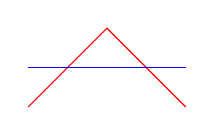
\begin{tikzpicture}
    \draw[red] (0,0) -- (1,1) -- (2,0);
    \draw[blue] (0,0.5) -- (2,0.5);
\end{tikzpicture}
\end{codeexample}
	We have two lines, both start on the left-hand-side. Our goal is to get a new path consisting of the intersections segments on the lower part of the picture, i.e.\ we would like to see
\begin{codeexample}[]
\begin{tikzpicture}
	% this is our goal - but computed automatically.
    \draw[black] (0,0) -- (0.5,0.5) -- (1.5,0.5) -- (2,0);
\end{tikzpicture}
\end{codeexample}
	
	In order to let |fillbetween| compute the target path, we assign names to the input paths, compute the intersections -- and recombined them using |\pgfcomputeintersectionsegments|:

\begin{codeexample}[vbox]
\begin{tikzpicture}[line join=round,x=3cm,y=3cm]
    \draw[name path=first,red] (0,0) -- (1,1) -- (2,0);
    \draw[name path=second,blue] (0,0.5) -- (2,0.5);

	% from 'name path' to softpaths...
	\tikzgetnamedpath{first}
	\let\A=\pgfretval
	\tikzgetnamedpath{second}
	\let\B=\pgfretval

	% compute intersections using the PGF intersection lib...
	\pgfintersectionofpaths{\pgfsetpath\A}{\pgfsetpath\B}%

	% ... and compute the intersection *segments* for both input
	% paths...
	\pgfcomputeintersectionsegments1
	\pgfcomputeintersectionsegments2

	% ... recombine the intersection segment paths!
	\pgfgetintersectionsegmentpath{1}{0}% path 1, segment 0
	\pgfsetpathandBB\pgfretval% this starts a new path
	\pgfgetintersectionsegmentpath{2}{1}% path 2, segment 1
	\pgfpathreplacefirstmoveto\pgfretval% connect, not move. Try to eliminate this line to see the effect
	\pgfaddpathandBB\pgfretval% append
	\pgfgetintersectionsegmentpath{1}{2}%
	\pgfpathreplacefirstmoveto\pgfretval
	\pgfaddpathandBB\pgfretval
	\pgfsetlinewidth{3}
	\pgfsetcolor{black}
	\pgfusepath{stroke}
\end{tikzpicture}
\end{codeexample}
	Note that this operates on a relatively low level. However, you can easily insert these statements into a |\pgfextra| in order to embed it into \tikzname. This allows access to any \tikzname\ options, including |decorate|:
\begin{codeexample}[vbox]
\begin{tikzpicture}[line join=round,x=3cm,y=3cm]
    \draw[name path=first,red] (0,0) -- (1,1) -- (2,0);
    \draw[name path=second,blue] (0,0.5) -- (2,0.5);

	\draw[orange,
		decorate,decoration={
			footprints,
			foot of=bird,
			stride length=15pt,
			foot sep=2pt,
			foot length=6pt},
	]
	\pgfextra
		% from 'name path' to softpaths...
		\tikzgetnamedpath{first}
		\let\A=\pgfretval
		\tikzgetnamedpath{second}
		\let\B=\pgfretval
		%
		% compute intersections using the PGF intersection lib...
		\pgfintersectionofpaths{\pgfsetpath\A}{\pgfsetpath\B}%
		%
		% ... and compute the intersection *segments* for both input
		% paths...
		\pgfcomputeintersectionsegments1
		\pgfcomputeintersectionsegments2
		%
		% ... recombine the intersection segment paths!
		\pgfgetintersectionsegmentpath{1}{0}% path 1, segment 0
		\pgfsetpathandBB\pgfretval% this starts a new path
		\pgfgetintersectionsegmentpath{2}{1}% path 2, segment 1
		\pgfpathreplacefirstmoveto\pgfretval% connect, not move
		\pgfaddpathandBB\pgfretval% append
		\pgfgetintersectionsegmentpath{1}{2}%
		\pgfpathreplacefirstmoveto\pgfretval
		\pgfaddpathandBB\pgfretval
	\endpgfextra
	;
\end{tikzpicture}
\end{codeexample}
\end{command}

\begin{command}{\pgfgetintersectionsegmentpath\marg{1 or 2}\marg{index}}
	Defines |\pgfretval| to contain the desired path segment as softpath.

	The result has the same quality as a path returned by |\pgfgetpath| and can be used by means of |\pgfsetpath|, |\pgfsetpathandBB|, or |\pgfaddpathandBB|.

	The value \meta{1 or 2} resembles the argument of a preceding call to |\pgfcomputeintersectionsegments|: it identifies which of the two paths for which intersections have been computed is to be selected.

	The second argument \meta{index} is a number $0 \le i < N$ where $N$ is the total number of computed segments. The total number of computed segments is returned by |\pgfcomputeintersectionsegments|.

	This macro is part of |fillbetween|.
\end{command}

\begin{command}{\tikzgetnamedpath\marg{string name}}
	Defines |\pgfretval| to contain the softpath associated with \meta{string name}. The \meta{string name} is supposed to be the value of |name path| or |name path| global.

	The resulting value is a softpath, i.e.\ it has the same quality as those returned by |\pgfgetpath|.

	This macro is part of |fillbetween|.
\end{command}

\begin{command}{\pgfgetpath\marg{\textbackslash softpathmacro}}
	Stores the current softpath into the macro \meta{\textbackslash softpathmacro}.

	See also |\tikzgetnamedpath|.

	This macro is part of \pgfname.
\end{command}

\begin{command}{\pgfsetpath\marg{\textbackslash softpathmacro}}
	Replaces the current softpath from the macro \meta{\textbackslash softpathmacro}.

	This does not update any bounding boxes. Note that this takes a soft--path as it is, no transformation will be applied. The only way to modify the path and its coordinates is a decoration or a canvas transformation.

	This macro is part of \pgfname.
\end{command}
\begin{command}{\pgfaddpath\marg{\textbackslash softpathmacro}}
	Appends the softpath from the macro \meta{\textbackslash softpathmacro} to the current softpath.

	This does not update any bounding boxes. Note that this takes a soft--path as it is, no transformation will be applied. The only way to modify the path and its coordinates is a decoration or a canvas transformation.

	This macro is part of \pgfname.
\end{command}

\begin{command}{\pgfsetpathandBB\marg{\textbackslash softpathmacro}}
	Replaces the current softpath from the macro \meta{\textbackslash softpathmacro}.

	This updates the picture's bounding box by the coordinates found inside of \meta{\textbackslash softpathmacro}. Aside from that, the same restrictions as for |\pgfsetpath| hold here as well.

	This macro is part of |fillbetween|.
\end{command}

\begin{command}{\pgfaddpathandBB\marg{\textbackslash softpathmacro}}
	Appends the softpath of macro \meta{\textbackslash softpathmacro} to the current softpath.

	This updates the picture's bounding box by the coordinates found inside of \meta{\textbackslash softpathmacro}. Aside from that, the same restrictions as for |\pgfsetpath| hold here as well.

	This macro is part of |fillbetween|.
\end{command}

\begin{command}{\pgfpathreplacefirstmoveto\marg{\textbackslash softpathmacro}}
	Takes a macro containing a softpath on input, replaces its first moveto operation by a lineto operation and returns it as |\pgfretval|.

	The argument \meta{\textbackslash softpathmacro} is one which can be retrieved by |\pgfgetpath|.

	This macro is part of |fillbetween|.
\end{command}

\begin{command}{\pgfintersectionofpaths\marg{first}\marg{second}}
	The \pgfname\ basic layer command to compute intersections of two softpaths. The arguments \meta{first} and \meta{second} are supposed to set paths, i.e.\ they should contain something like |\pgfsetpath{\somesoftpath}|.

	Results are stored into variables of the current scope.

	This macro is part of \pgfname.
\end{command}

\begin{command}{\pgfpathcomputesoftclippath\marg{\textbackslash inputsoftpath}\marg{\textbackslash softclippath}}
	Does the work for |soft clip|: it computes the soft--clip--path of \meta{\textbackslash inputsoftpath} when it is clipped against \meta{\textbackslash softclippath}.
	
	The algorithm has been tested and written for rectangular soft clip paths. It will accept complicated clip paths, and might succeed with some of them. Nevertheless, rectangular soft clip paths are the ones which are supported officially.

	See |soft clip| for details.
\end{command}
\endgroup
